% chap1.tex
\part{서론}
\label{part:introduction}

% ---------------------------------------------------------------------------- %
%                                  NEW SECTION                                 %
% ---------------------------------------------------------------------------- %

\chapter{개발 배경 및 원리}

\section{동적 시뮬레이션 기반 그린리모델링 의사결정 지원도구}

 그린리모델링은 기술간의 교호작용을 고려할 수 있는 동적 시뮬레이션 도구가 필요하다.
 하지만 EnergyPlus는 ...하여 그린리모델링 사업에서 실제로 쓰이기에는 부적합하기 때문에, 요구, ...한 시뮬레이터가 요구된다.

% ---------------------------------------------------------------------------- %
%                                  NEW SECTION                                 %
% ---------------------------------------------------------------------------- %

\section{\simulator의 접근 및 철학}

\subsection{원칙}
ECO2 입력 수준 만큼의 노력으로 high-fidelity 동적 시뮬레이션 가능하게 하는 걸 목적으로 하여, 아래 원칙 하에서 개발하였다.

\begin{itemize}
  \item 기존에 국내에서 쓰이던 건물 에너지 평가 도구의 입력 수준과 유사
  \item EnergyPlus 엔진을 사용하여 건물의 동적 거동 상세하게 모사
  \item 기축건물에서 사용자가 얻기 어렵지만, 동적 시뮬레이터에서 요구하는 것들 가정 (normative dynamic)
  \item ASHRAE F., 건축물에너지효율등급인증규정 등 국내외 기준 참고하여 표준적인 시뮬레이션이 가능
\end{itemize}

\subsection{다른 도구들과의 관계}
\subsubsection{EnergyPlus, DesignBuilder}
\simulator\는 EnergyPlus의 wrapper로 볼 수 있다. EnergyPlus는 엔진의 역할, DesignBuilder가 그걸 포장하는 툴인데, \simulator~도 비슷한 관점에서 개발되었다. 단, DesignBuilder는 높은 자유도를 거의 그대로 보장하고 사용 가능한 dataset도 그냥 열린 반면에, \simulator\는 국내 실정과 기축건물의 그린리모델링이라는 상황에 적합하게 커스터마이징하여, 그린리모델링 사업에 적합하게 사용 가능하다.

\subsubsection{ClimateStudio, Honeybee}
둘 다 EnergyPlus의 앞서 언급한 DesignBuilder와 같은 wrapper인데, Raw-level에서의 수정도구인 DesignBuilder보다는 좀 더 graphical code 개념도 쓰고 해서 좀 더 구조적인 모델링이 가능하다. \simulator~의 자료구조와 python 코드상의 구조는 두 프로그램의 자료구조를 참고하여 개발되었다.

\subsubsection{ECO2(-OD)}
\simulator\는 ECO2의 입력 수준을 많이 넘지 않는 것을 원칙으로 하고 있기 때문에, 입력변수의 종류와 그 상세함의 정도는 ECO2 및 ECO2-OD를 참고하여 결정하였다. 특히 실 단위 부하를 계산하는 ECO2의 데이터베이스 등을 많이 참고하였다.

% ---------------------------------------------------------------------------- %
%                                  NEW SECTION                                 %
% ---------------------------------------------------------------------------- %

\section{\simulator의 개요 및 역할}

\simulator\는 사용자의 간단한 입력데이터를 \ep 실행이 가능한 형태로 변환하는 도구로 이해할 수 있다 (그림 \ref{fig:package_function}). 그 변환 과정은 python이 매개한다.

\begin{defaultfigure}
  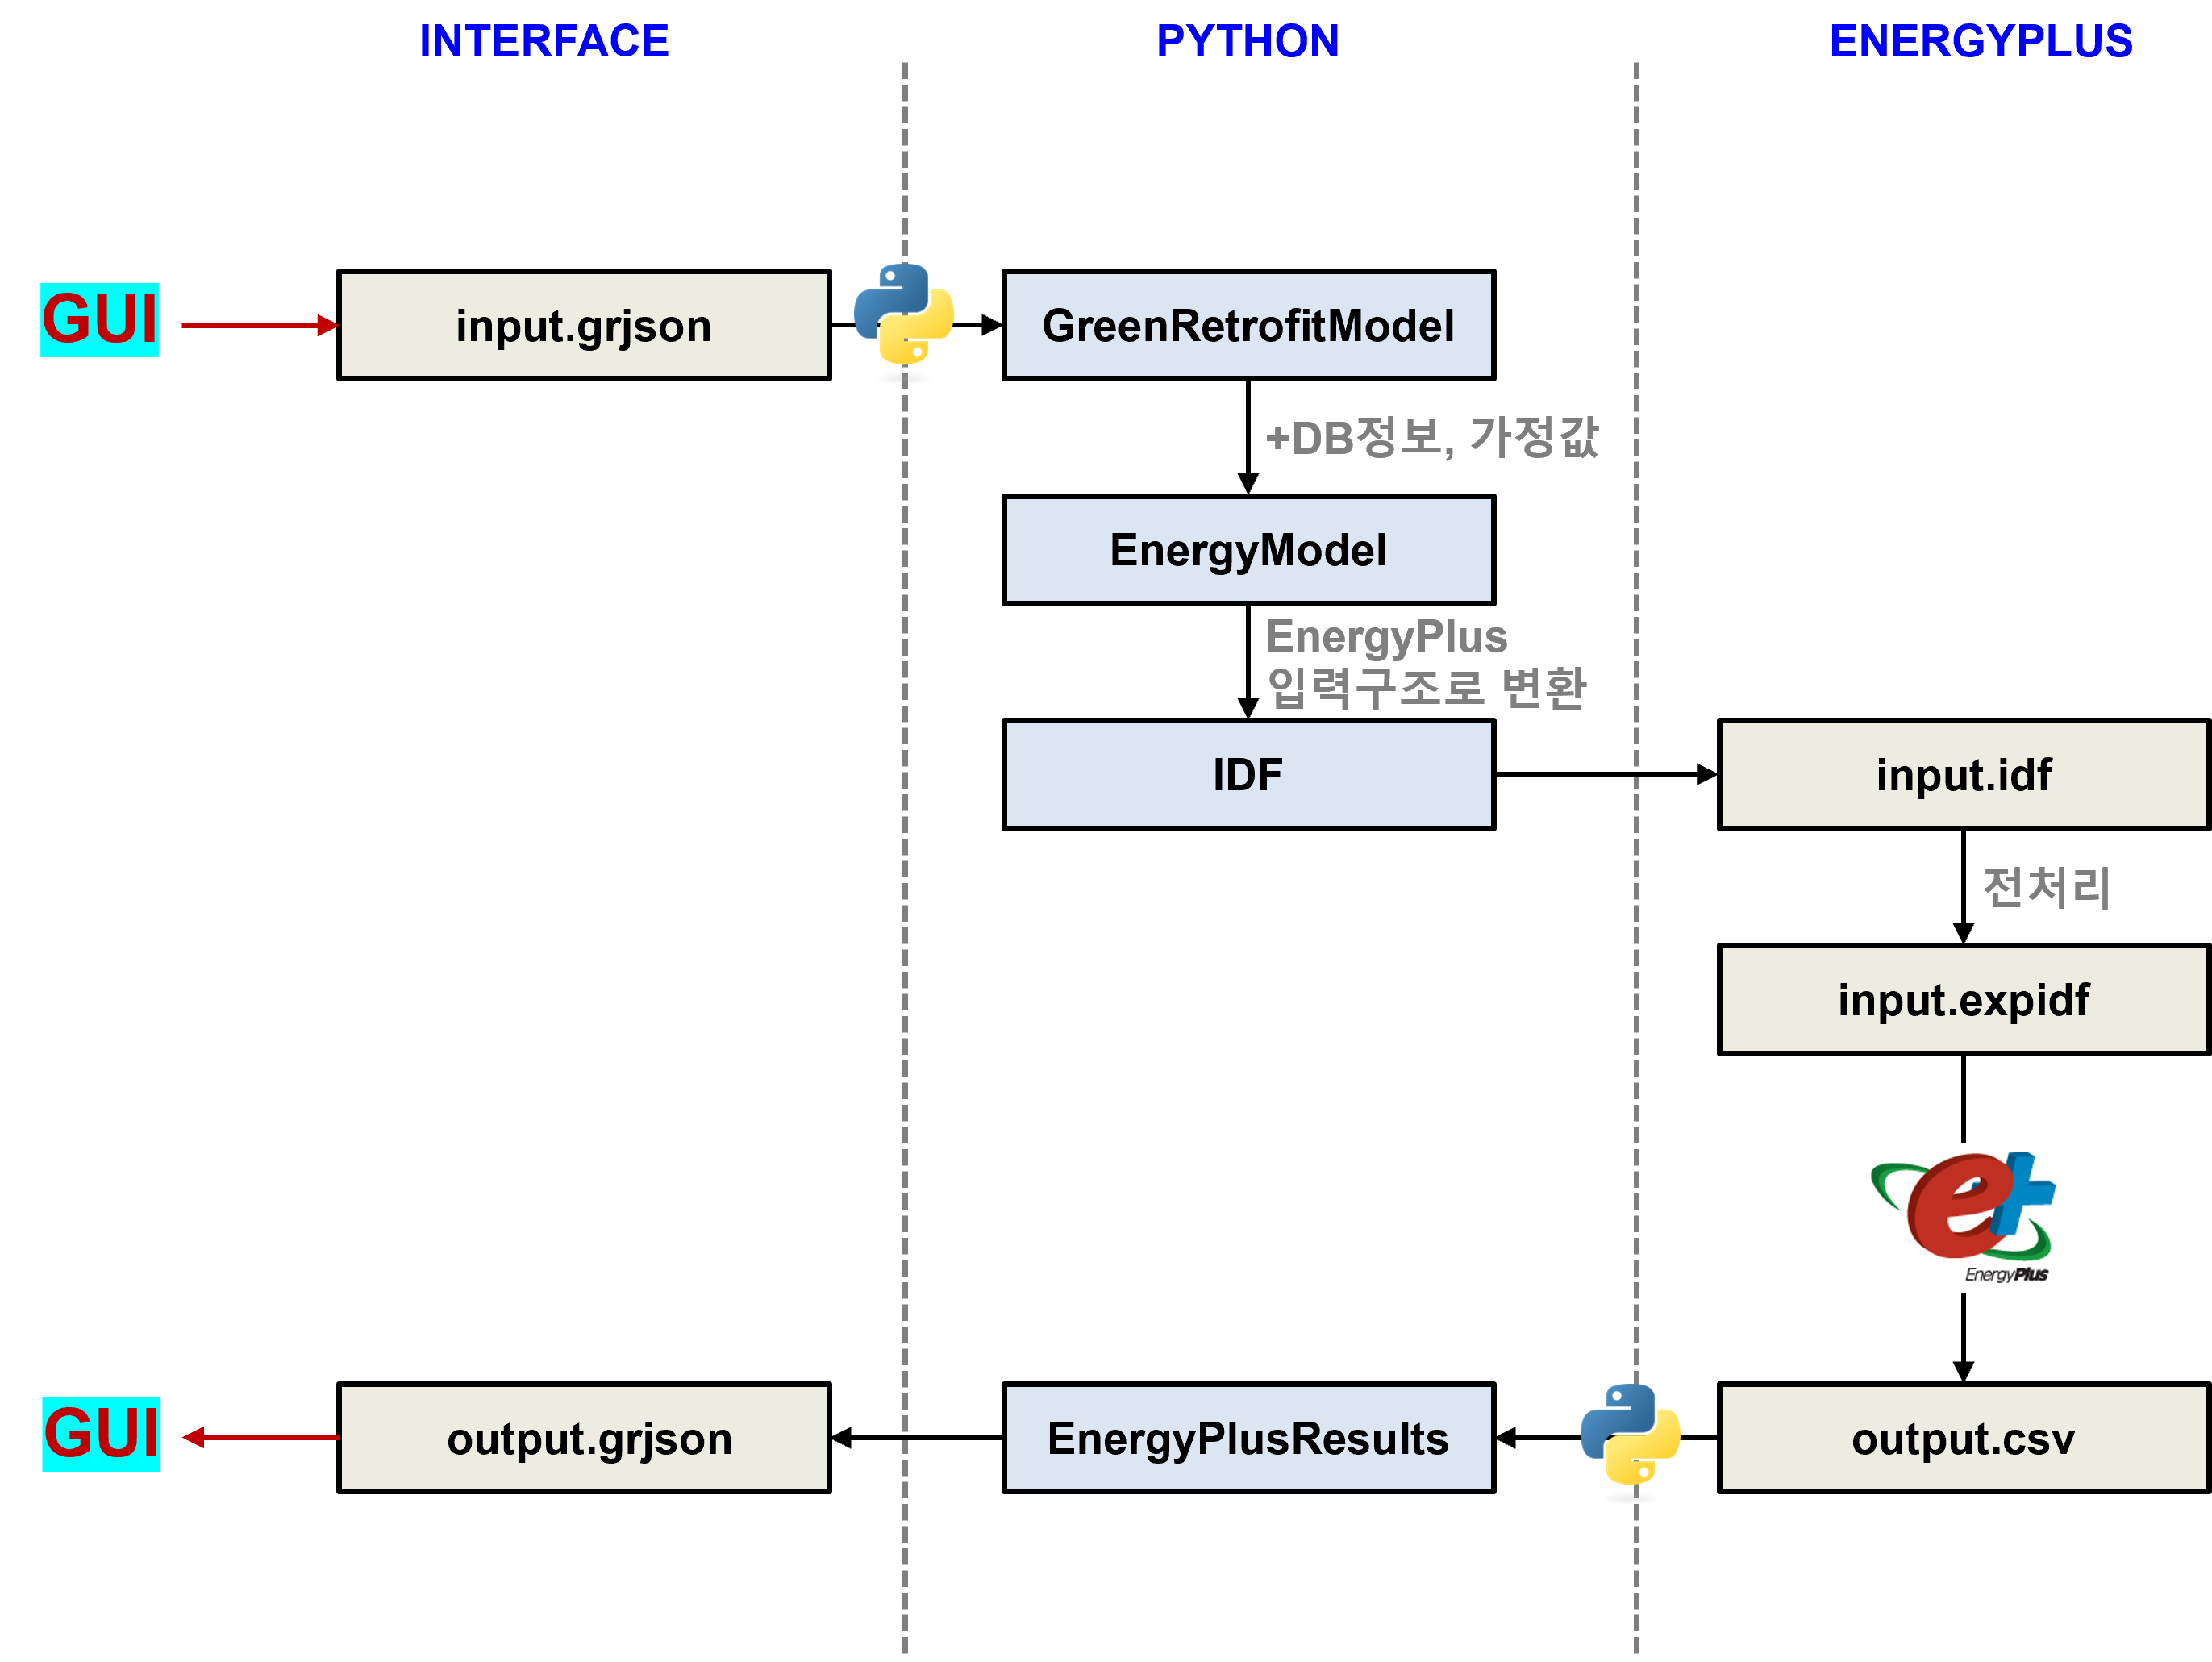
\includegraphics[width=\textwidth]{GRSimulator의 실체.png}
  \caption{\simulator에서 데이터가 전달되는 과정}
  \label{fig:package_function}
\end{defaultfigure}
